% !TEX encoding = UTF-8 Unicode

% Geoscientific Model Development (gmd)
\documentclass[gmd, manuscript]{copernicus}

% packages
\usepackage{tabu}
\usepackage{booktabs}
\usepackage{graphicx}
\usepackage[export]{adjustbox}
\usepackage[utf8]{inputenc}
\usepackage{listings}
\usepackage[percent]{overpic}

\begin{document}

\title{\lowercase{r.sim.terrain 1.0}: a landscape evolution model with dynamic hydrology} 

\Author[1]{Brendan Alexander}{Harmon}
\Author[2,3]{Helena}{Mitasova}
\Author[2,3]{Anna}{Petrasova}
\Author[2,3]{Vaclav}{Petras}

\affil[1]{Robert Reich School of Landscape Architecture, Louisiana State University, Baton Rouge, Louisiana, USA}
\affil[2]{Center for Geospatial Analytics, North Carolina State University, Raleigh, North Carolina, USA}
\affil[3]{Department of Marine, Earth, and Atmospheric Sciences, North Carolina State University, Raleigh, North Carolina, USA}

\runningtitle{\lowercase{r.sim.terrain 1.0}: a landscape evolution model with dynamic hydrology} 

\runningauthor{Brendan Harmon}

\correspondence{Brendan Harmon (baharmon@lsu.edu)}

\received{}
\pubdiscuss{}
\revised{}
\accepted{}
\published{}

\firstpage{1}

\maketitle

\begin{abstract}
While there are numerical landscape evolution models
that simulate how steady state flows of water and sediment
reshape topography over long periods of time, 
r.sim.terrain is the first to 
simulate short-term topographic change 
for both steady state and dynamic flow regimes
across a range of spatial scales.
This free and open source, 
GIS-based topographic evolution model
uses empirical models for soil erosion
and a physics-based model
for shallow overland water flow and soil erosion 
to compute short-term topographic change. 
This model uses either a steady state 
or unsteady representation of overland flow
to simulate how overland sediment mass flows reshape topography
for a range of hydrologic soil erosion regimes
based on topographic, land cover, soil, and rainfall parameters. 
As demonstrated by a case study 
for Patterson Branch subwatershed
on the Fort Bragg military installation in North Carolina,
r.sim.terrain simulates the development of 
fine-scale morphological features including 
ephemeral gullies, rills, and hillslopes.
Applications include land management, erosion control,
landscape planning, and landscape restoration. 
\end{abstract}

\copyrightstatement{...}

% --------- INTRO FIGURE ---------

\begin{figure}%[H]
\center
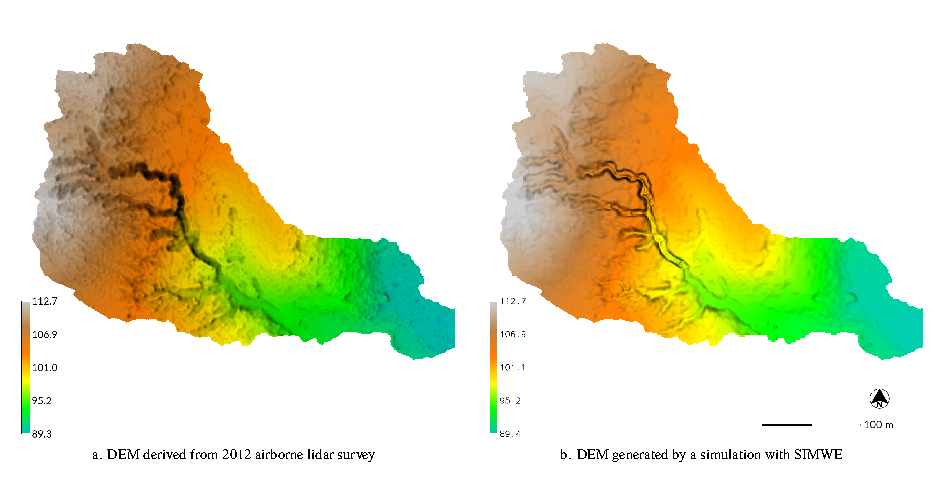
\includegraphics[width=\textwidth,height=0.925\textheight,keepaspectratio]{figures/evolution.pdf}
\caption{
The digital elevation model (DEM) 
(a) before and (b) after
simulated landscape evolution with r.sim.terrain 
for a subwatershed of Patterson Branch, Fort Bragg, NC, USA. 
(a) The before DEM was generated from an airborne lidar survey in 2012. 
This simulation used the SIMWE model
for a 120~\unit{min} rainfall event with 50~\unit{mm~hr}$^{-1}$
for a variable erosion-deposition regime at steady state.
(b) In the evolved DEM 
the gully channel has widened 
with depositional ridges forming along its thalweg.}
\label{fig:evolution}
\end{figure}

% --------- BODY ---------

\introduction
Landscape evolution models represent how the surface of the earth changes 
over time in response to physical processes. 
Most studies of landscape evolution have been descriptive, 
but a number of numerical landscape evolution models 
have been developed that simulate elevational change over time 
\citep{Tucker2010,Temme2013}. 
% numerical models
Numerical landscape evolution models such as the 
Geomorphic - Orogenic Landscape Evolution Model (GOLEM) 
\citep{Tucker1994},
CASCADE \citep{Braun1997},
the Channel-Hillslope Integrated Landscape Development (CHILD) model 
\citep{Tucker2001},
CAESAR \citep{Coulthard2002,Coulthard2012},
SIBERIA \citep{Willgoose2005},
LAPSUS \citep{Schoorl2000,Schoorl2002},
and r.landscape.evol \citep{Barton2010}
simulate landscape evolution driven primarily by steady state flows over long temporal scales.
% recent development
\href{http://landlab.github.io/}{Landlab},
a new Python library for numerically modeling Earth surface processes
\citep{Hobley2017},
has components for simulating landscape evolution such as the 
Stream Power with Alluvium Conservation and Entrainment (SPACE) 
model \citep{Shobe2017}.
% gis-based models
While Geographic Information Systems (GIS)
support efficient data management, 
spatial and statistical modeling and analysis, 
and visualization,
there are few GIS-based soil erosion models (see Table~\ref{table:erosion_models})
or landscape evolution models.
% r.terradyn
\cite{Thaxton2004} developed the model r.terradyn 
as a GRASS GIS shell script module 
to simulate terrain evolution 
by steady state net erosion-deposition rates
estimated by the Simulation of Water Erosion (SIMWE) model \citep{Mitas1998}
and gravitational diffusion. 
% r.landscape.evol
\cite{Barton2010} developed a long term landscape evolution model
in GRASS GIS called r.landscape.evol that integrates 
the Unit Stream Power Erosion Deposition (USPED) model,
fluvial erosion, and gravitational diffusion.
r.landscape.evol has been used to simulate the impact 
of prehistoric settlements on Mediterranean landscapes.
% research questions
In spite of the recent progress in landscape evolution modeling and monitoring, 
there are still major research questions 
to address in the theoretical foundations of erosion modeling 
such as how erosional processes scale over time and space 
and how sediment detachment and transport interact \citep{Mitasova2013}. 
% dynamic evolution
While most numerical landscape evolution models 
simulate erosion processes at steady state, peak flows,
short-term erosional processes like gully formation 
can be driven by unsteady, dynamic flow
with significant morphological changes happening before flows reach steady state. 
A landscape evolution model with dynamic water and sediment flow
is needed to study fine-scale spatial 
and short-term erosional processes
such as gully formation and the development of microtopography. 

% steady state versus dynamic
At the beginning of a rainfall event 
overland water flow is unsteady -- 
its depth changes at a variable rate over time and space. 
If the intensity of rainfall continues to change throughout the event
then the flow regime will remain dynamic. 
% steady state
If, however, overland flow reaches a peak rate
then the hydrologic regime is considered to be at steady state.
At steady state:
% steady state eq.
\begin{equation}
\label{eq:steady_state}
{\partial h(x,y,t) \over \partial t} = 0
\end{equation}
%
{\small
\noindent
where: \\
\noindent
\hspace*{0.5em} $(x,y)$ is the position [\unit{m}]\\
\hspace*{0.5em} $t$ is the time [\unit{s}]\\
\hspace*{0.5em} $h(x,y,t)$ is the depth of overland flow [\unit{m}].\\
}

% gully formation
Gullies are eroded, steep banked channels 
formed by ephemeral, concentrated flows of water.
A gully forms when overland waterflow
converges in a knickzone
-- a concave space with steeper slopes than its surroundings 
\citep{Zahra2017} -- 
during intense rainfall events.  
When the force of the water flow concentrated in the knickzone
is enough to detach and transport large amounts of sediment,
an incision begins to form at the apex of the knickzone 
-- the knickpoint or headwall.
As erosion continues the knickpoint begins to migrate upslope
and the nascent gully channel widens,
forming steep channel banks. 
Multiple incisions initiated by different knickpoints 
may merge into a gully channel
and multiple channels may merge 
into a branching gully system \citep{Mitasova2013}. 
% detachment limited
This erosive process is dynamic; 
the morphological changes drive further changes 
in a positive feedback loop.
When the gully initially forms 
the soil erosion regime should be detachment capacity limited
with the concentrated flow of water in the channel of the gully 
detaching large amounts of sediment 
and transporting it to the foot of the gully, 
potentially forming a depositional fan.
% variable erosion-deposition
If the intensity of rainfall decreases
and transport and detachment capacity 
approach a balance, 
then the soil erosion regime may switch to 
a variable erosion-deposition regime,
in which soil is eroded and deposited 
in a spatially variable pattern.
Subsequent rainfall events may trigger further 
knickpoint formation and upslope migration, 
channel incision and widening, and
depositional fan and ridge formation. 
Between high intensity rainfall events, 
lower intensity events and gravitational diffusion
may gradually smooth the shape of the gully. 
% transport limited
Eventually, if detachment capacity 
significantly exceeds transport capacity
and the regime switches to transport capacity limited, 
the gully may fill with sediment
as soil continues to be eroded, 
but can not be transported far. 

% gully monitoring
Gully erosion rates and evolution
can be monitored in the field 
or modeled on the computer. 
% field methods
Field methods include
dendrogeomorphology \citep{Malik2008} and 
permanent monitoring stakes for recording erosion rates, 
extensometers for recording mass wasting events, 
weirs for recording water and suspended sediment discharge rates, 
and time series of surveys using 
total station theodolites \citep{Thomas2004},
unmanned aerial systems (UAS) \citep{Jeziorska2016,Kasprak2019,Yang2019},
airborne lidar \citep{Perroy2010,Starek2011}, 
and terrestrial lidar \citep{Starek2011,Bechet2016,Goodwin2016,Telling2017}.
% high resolution topographic data
With terrestrial lidar, airborne lidar, and 
UAS photogrammetry
there is now sufficient resolution topographic data 
to morphometrically analyze and 
numerically model fine-scale landscape evolution in GIS
including processes such as gully formation 
and the development of microtopography. 
% gully simulation
Gully erosion has been simulated with 
RUSLE2-Raster (RUSLER)
in conjunction with the Ephemeral Gully Erosion Estimator (EphGEE)
\citep{Dabney2014},
while gully evolution
has been simulated for detachment capacity limited erosion regimes
with the Simulation of Water Erosion (SIMWE) model
\citep{Koco2011, Mitasova2013}. 
Now numerical landscape evolution models 
that can simulate 
steady state and unsteady flow regimes
and can dynamically switch between soil erosion regimes 
are needed to study 
fine-scale spatial and short-term erosional processes.

% aim
The numerical landscape evolution model 
r.sim.terrain was developed to 
simulate the spatiotemporal evolution of landforms
caused by shallow overland water and sediment flows
at spatial scales ranging from
square meters to kilometers
and temporal scales ranging from minutes to years. 
% objectives
This open source, GIS-based landscape evolution model can
simulate either steady state or unsteady flow regimes,
dynamically switch between soil erosion regimes, and
simulate the evolution of fine-scale morphological features 
such as ephemeral gullies
(Figure~\ref{fig:evolution}).
% questions
It was designed as a research tool for
studying how erosional processes scale over time and space,
comparing empirical and process-based models, 
comparing steady state and unsteady flow regimes, and
studying the role of unsteady flow regimes
in fine-scale morphological change. 
% testing
r.sim.terrain was tested with 
a subwatershed scale (450~\unit{m}$^{2}$) case study
and the simulations were compared against 
a time-series of airborne lidar surveys.

\section{r.sim.terrain}

% --------- CONCEPT MODEL ---------

\begin{figure}%[H]
\center
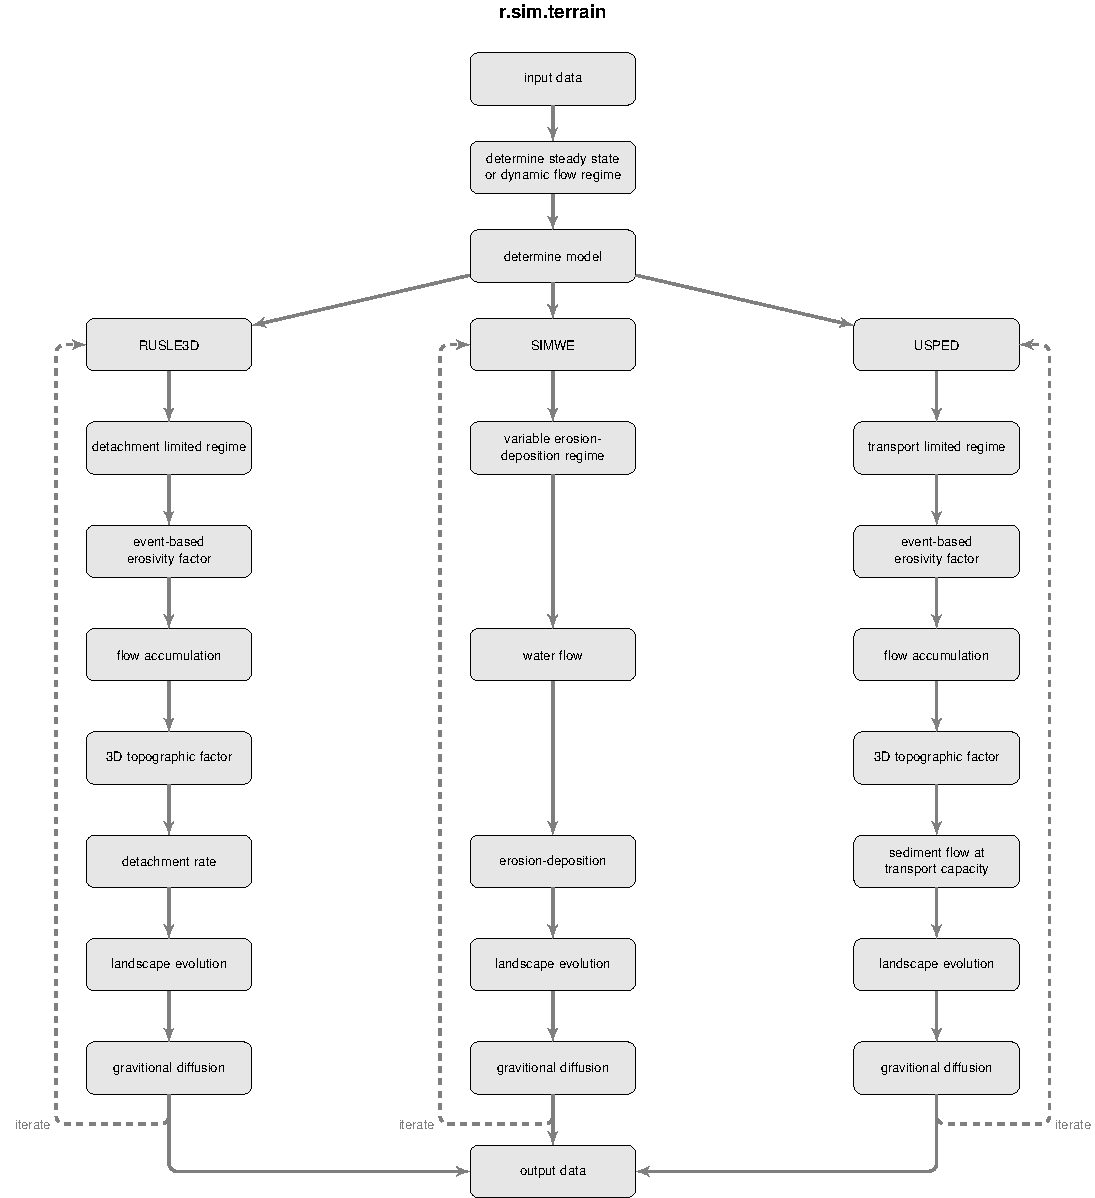
\includegraphics[width=\textwidth,keepaspectratio]{figures/concept.pdf}
\caption{Conceptual diagram for r.sim.terrain.}
\label{fig:evolution}
\end{figure}

% ---------------------------------

The process-based, spatially distributed 
landscape evolution model r.sim.terrain
simulates topographic changes
caused by shallow, overland water flow
across a range of spatiotemporal scales and soil erosion regimes
using either
the Simulated Water Erosion (SIMWE) model, 
the 3-Dimensional Revised Universal Soil Loss Equation (RUSLE 3D) model,
or the Unit Stream Power Erosion Deposition (USPED) model (Figure~\ref{fig:evolution}).  
The r.sim.terrain model
can simulate either steady state or dynamic flow regimes.
% simwe
SIMWE is a physics-based simulation
that uses a Monte Carlo path sampling method
to solve the water and sediment flow equations
for detachment limited, transport limited, and variable erosion-deposition 
soil erosion regimes 
\citep{Mitas1998,Mitasova2004}. 
With SIMWE 
r.sim.terrain
uses the modeled flow of sediment 
-- a function of water flow and soil detachment and transport parameters -- 
to estimate net erosion and deposition rates. 
% rusle3d
RUSLE3D is an empirical equation for estimating soil erosion rates
in detachment capacity limited soil erosion regimes 
\citep{Mitasova1996,Mitasova2013}. 
%
With RUSLE3D r.sim.terrain
uses an event-based rainfall erosivity factor, 
soil erodibility factor, landcover factor, and 3D topographic factor
-- a function of slope and flow accumulation --
to model soil erosion rates. 
% usped
USPED is a semi-empirical equation for net erosion and deposition 
in transport capacity limited soil erosion regimes 
\citep{Mitasova1996,Mitasova2013}. 
With USPED r.sim.terrain uses an event-based rainfall erosivity factor, 
soil erodibility factor, landcover factor, and a topographic sediment transport factor
to model net erosion or deposition rates as the divergence of sediment flow. 
% evolution
For each of the models 
topographic change is derived at each time step
from the net erosion-deposition rate
and gravitational diffusion.
% regimes
Depending on the input parameters, 
r.sim.terrain simulations with SIMWE 
can represent variable soil erosion-deposition regimes, 
including prevailing detachment capacity limited 
or prevailing transport capacity limited regimes.

% capabilities
The r.sim.terrain model
can simulate the evolution of gullies
including processes such as 
knickpoint migration,
channel incision, 
channel widening, 
aggradation, 
scour pit formation,
depositional ridge formation
along the thalweg of the gully,
and depositional fan formation at the foot of the gully. 
% applications
Applications include 
geomorphological research,
erosion control, 
landscape restoration, 
and scenario development 
for landscape planning and management.
% scale
This model can simulate landscape evolution 
over a wide range of spatial scales 
from small watersheds 
less than ten square kilometers
with SIMWE
to regional watersheds
of hundreds of square kilometers
with USPED or RULSE3D,
although it does not model fluvial processes. 
It has been used at resolutions ranging from sub-meter to 30~\unit{m}.
% implementation
The model has been implemented 
as a Python add-on module 
for the free, open source
\href{https://grass.osgeo.org/}{Geographic Resources Analysis Support System (GRASS) GIS}
\citep{GRASS}. 
The source code is available at 
\url{https://github.com/baharmon/landscape\_evolution} 
under the GNU General Public License v2.
% parallel processing
It supports multithreading and parallel processing
to efficiently compute simulations 
using large, high resolution topographic datasets.
%
The landscape evolution model 
can be installed in GRASS GIS as an add-on module 
with the command: 
\begin{verbatim}
g.extension extension=r.sim.terrain
\end{verbatim}

% -------------------------- TABLE OF MODELS -----------------------------

% table of erosion models
\begin{table*}
\small
\caption{Geospatial soil erosion models}
\begin{tabu} to \textwidth {XXXXXl}
\toprule
Model & Spatial scale &  Temporal scale & Representation & Implementation & Reference\\
\midrule
RUSLE3D & regional & continuous & raster & map algebra & \citep{Mitasova1996}\\
USPED & watershed & continuous & raster & map algebra & \citep{Mitasova1996}\\
\href{https://grass.osgeo.org/grass74/manuals/r.sim.sediment.html}{SIMWE} & watershed & event -- & raster & \href{https://grass.osgeo.org/grass74/manuals/r.sim.sediment.html}{GRASS modules} & \citep{Mitas1998}\\
&& continuous\\
\href{http://geowepp.geog.buffalo.edu/}{GeoWEPP} & watershed & continuous & raster & \href{http://geowepp.geog.buffalo.edu/}{ArcGIS module} & \citep{Flanagan2013}\\
\href{https://www.tucson.ars.ag.gov/agwa/}{AGWA} & watershed & event -- & vector & \href{https://www.tucson.ars.ag.gov/agwa/}{ArcGIS module} & \citep{Guertin2015}\\
&& continuous\\
\href{https://blog.utwente.nl/lisem/}{openLISEM} & watershed & event & raster & \href{https://blog.utwente.nl/lisem/}{PCRaster script} & \citep{Roo1996}\\
\href{https://github.com/landlab/}{Landlab} & watershed & event -- & raster + mesh & \href{https://github.com/landlab/}{Python library} & \citep{Hobley2017}\\
&& continuous\\

\bottomrule
\\
\end{tabu}
\label{table:erosion_models}
\end{table*}

% -------------------------- MODEL FIGURE -------------------------

% model figure
\begin{figure}
\center
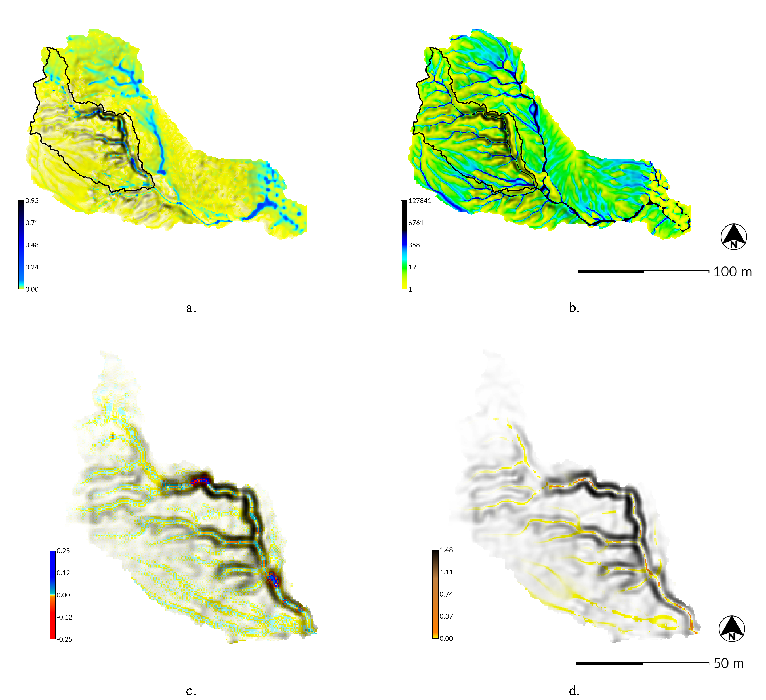
\includegraphics[width=\textwidth,height=0.95\textheight,keepaspectratio]{figures/models.pdf}
\caption{Water and sediment flows 
modeled by (a \& c) SIMWE and (b \& d) RUSLE3D with spatially variable landcover 
for (a \& b) a subwatershed and (c \& d) drainage area of Patterson Branch, Fort Bragg, NC.
(a) Water depth [m] simulated by SIMWE for a 10~\unit{min} event with 50~\unit{mm~hr}$^{-1}$ in the subwatershed.
(b) Flow accumulation for RUSLE3D in the subwatershed.
(c) Erosion and deposition [\unit{kg~m}$^{-2}$~\unit{s}$^{-1}$] simulated by SIMWE in drainage area 1.
(d) Erosion [\unit{kg~m}$^{-2}$~\unit{s}$^{-1}$] modeled by RUSLE3D in drainage area 1.
}
\label{fig:models}
\end{figure}

% --------------- MATH FOUNDATIONS OF THE MODEL ------------------

\subsection{Landscape evolution}

Landscape evolution in r.sim.terrain 
is driven by the change in the elevation surface 
caused by soil erosion and deposition.
During storm events overland flow erodes soil, 
transports sediment across landscape, and 
under favorable conditions deposits the sediment. 
Gravitational diffusion, 
applied to the changed elevation surface, 
simulates the smoothing effects 
of localized soil transport between events.

\subsubsection{Elevation change} 
Assuming negligible uplift, the change in elevation over time 
is described by the continuity of mass equation 
expressed as the divergence of sediment flow  \citep{Tucker2001}:
% landscape evolution equation
\begin{equation}
\label{eq:evolution} 
{\partial z \over \partial t } = \left (-\nabla \cdot {\bf q_s} \right ) ~ \rho_s^{-1} = d_s ~ \rho_s^{-1} 
\end{equation}
{\small
where: \\
\noindent
\hspace*{0.5em} $z$ is elevation [\unit{m}] \\
\hspace*{0.5em} $t$ is time [\unit{s}] \\
\hspace*{0.5em} ${\bf q_s}$ is sediment flow per unit width (vector) [\unit{kg~m}$^{-1}$~\unit{s}$^{-1}$]\\
\hspace*{0.5em} $d_s$ is the net erosion-deposition rate [\unit{kg~m}$^{-2}$~\unit{s}$^{-1}$]\\
\hspace*{0.5em} $\rho_s$ is sediment mass density [\unit{kg~m}$^{-3}$].\\
}
In r.sim.terrain
the net erosion-deposition rate $d_s$ driven by overland flow
is estimated at different levels of complexity based 
on the simulation mode selected by the user.
Gravitational diffusion is then applied to the changed topography 
to simulate the smoothing effects 
of localized soil transport between rainfall events.
The change in elevation due to gravitational diffusion
is a function of the sediment mass density,
the diffusion coefficient, and the Laplacian of the elevation
%-- i.e.~the sum of the second order derivatives of elevation
\citep{Thaxton2004}:
% change in elevation (m) = elevation (m) - (change in time (s) / sediment mass density (kg/m^3) * gravitational diffusion coefficient (m^2/s) * divergence (m^-1))
\begin{equation}
\label{eq:grav_diffusion} 
{\partial z \over \partial t } =  \varepsilon_g ~ \nabla^2 z 
\end{equation}
%HM this should be \nabla^2 z, \nabla is an operator so there should be a variable upon which it is applied
%HM see eq 4.41 in Thaxton, also from Willgoose, the second term
\noindent
where $\varepsilon_g$ is the diffusion coefficient [\unit{kg~m}$^{2}$~\unit{s}$^{-1}$].
%HM we can write $\varepsilon_g=c~\varepsilon$ where c[kg] to keep the diffusion coef units the same as in literature
%If it is the same time step we have
%\begin{equation}
%\label{eq:evolution_disc1} 
%z_{t + \Delta t} = z_t + \Delta z_s + \Delta z_g 
%\end{equation}
%if the time step advances we need two equations, something like this: or see Thaxton
%HM VERIFY whether this is acceptable

\noindent
The discrete implementation follows \cite{Thaxton2004}:
\begin{equation}
\label{eq:evolution_disc1} 
z_{t+ \Delta t_1} = z_t + \Delta z_s  
\end{equation}
\begin{equation}
\label{eq:evolution_disc2} 
z_{t+\Delta t_1+\Delta t_2} = z_{t+\Delta t_1} + \Delta z_g 
\end{equation}
{\small
where: \\
\noindent
\hspace*{0.5em} $\Delta z_s$ is elevation change [\unit{m}] caused by net erosion or deposition during time interval $\Delta t_1$ [\unit{s}]
(Eq.~\ref{eq:evolution})\\
\hspace*{0.5em} $\Delta z_g$ is the diffusion driven elevation change [\unit{m}] during time interval $\Delta t_1$ [\unit{s}] 
(Eq.~\ref{eq:grav_diffusion}).\\
}
%HM  we need to conclude this with reference to Thaxton? about delta z and stability of the solution
%and/or that t1 and t2 can be different 

\subsubsection{Erosion-deposition regimes}

%In general, the net erosion-deposition $d_s$ is obtained 
%by solving the sediment transport continuity equation
%which for the simpler, steady state case relates $d_s$ to the divergence 
%of sediment flow rate per unit width ${\bf q_s}$ [\unit{kg~m}$^{-1}$~\unit{s}$^{-1}$]:
%\begin{equation}
%\label{eq:steady_sed}
%d_s = \nabla\cdot {\bf q_s} 
%\end{equation}
Following experimental observations and qualitative arguments, 
\cite{Foster1977} proposed that the sum of 
the ratio of the net erosion-deposition rate $d_s$ 
to the detachment capacity  $D_c$  [\unit{kg~m}$^{-2}$~\unit{s}$^{-1}$] 
and the ratio of the sediment flow rate $q_s = |{\bf q_s}|$ 
to the sediment transport capacity $T_c$ [$\unit kg~m^{-1}~s^{-1}$]
is a conserved quantity (unity):
\begin{equation}
\label{eq:foster_law}
{d_s \over D_c} + {q_s \over T_c} = 1
\end{equation}
The net erosion and deposition rate $d_s$ can then be expressed 
as being proportional to the difference between
the sediment transport capacity $T_c$ 
and the actual sediment flow rate $q_s$:
\begin{equation}
\label{eq:sigma}
d_s = {D_c \over T_c}~\bigl( T_c - q_s\bigr)
\end{equation}
\noindent
This principle is used in several erosion models 
including the Water Erosion Prediction Project (WEPP) \citep{Flanagan2013} 
and SIMWE \citep{Mitas1998}. 

Using this concept it is possible to identify 
two limiting erosion-deposition regimes.
When $T_c >> D_c$ leading to $T_c >> q_s$, 
the erosion regime is detachment capacity limited and
net erosion is equal to the detachment capacity:
\begin{equation}
\label{eq:detachment_limited}
 d_s = D_c
\end{equation}
For this case the transport capacity of overland flow 
exceeds the detachment capacity 
and thus sediment flow, erosion, and sediment transport
are limited by the detachment capacity. 
Therefore, no deposition occurs.
%When rainfall intensity is very high ($i_r \geq 60 \unit{mm~hr}^{-1}$)
An example of this case is when a strong storm 
producing intense % high 
overland flow over compacted clay soils 
causes high capacity flows to transport light clay particles,
while the detachment of compacted soils is limited.
%
When $D_c >> T_c$, sediment flow is at sediment transport capacity $q_s = T_c$, 
leading to a transport capacity limited regime 
with deposition reaching its maximum extent for the given water flow. 
Net erosion-deposition is computed as the divergence of
transport capacity multiplied by a unit vector $\vec{s_0}$ 
in the direction of flow:
\begin{equation}
\label{eq:transport_limited}
 d_s = \nabla\cdot (T_c ~ \vec{s_0})
\end{equation}
%This would be the case when rainfall intensity is not very high ($i_r < 60 \unit{mm~hr}^{-1} $) and 
This case may occur, for example, during a moderate storm 
with overland flow over sandy soils 
with high detachment capacity, but low transport capacity.
%
For $0 < ({D_c / T_c}) < \infty$ 
the spatial pattern of net erosion-deposition is variable 
and depends on the difference between the sediment transport capacity 
and the actual sediment flow rate at the given location.

The detachment capacity $D_c $  and the sediment-transport capacity $T_c $  
are estimated using shear stress and stream power equations respectively
expressed as power functions of water-flow properties and slope angle.    
%For a given rainfall rate and surface roughness, these two variables can be derived from a DEM
%using topographic analysis functions to compute the slope 
%and flow-routing tools to compute the upslope contributing area 
%as an input for estimating unit water flow.
The relations between the topographic parameters 
of well known empirical equations for erosion modeling, 
such as USLE and stream power, were presented by \citet{Moore1986} 
and used to develop simple, GIS-based models for limiting erosion-deposition cases 
such as RUSLE3D and USPED \citep{Mitasova2001}.
The SIMWE model estimates $T_c$ and $D_c$ using modified 
equations and parameters developed for the WEPP model 
\citep{Flanagan2013,Mitasova2013}.

The simulation modes in r.sim.terrain include:
\begin{itemize}
  \item the process-based SIMWE model 
  for steady state and unsteady shallow overland flow 
  in variable erosion-deposition regimes
  with $d_s$ computed by solving the shallow water flow 
  and sediment transport continuity equations,
  \item the RUSLE3D model for detachment capacity limited cases
  with $d_s$ given by Eq.~(\ref{eq:detachment_limited}),
  \item and the USPED model for transport capacity limited regimes
  with $d_s$ given by Eq.~(\ref{eq:transport_limited}).
\end{itemize}

\noindent The following sections explain the computation of $d_s$ for these three modes in more detail.

% -------------------------- SIMWE -----------------------------
\subsection{Simulation of Water Erosion (SIMWE)} \label{simwe}
SIMWE is a physics-based simulation of shallow overland water and sediment flow
that uses a path sampling method to solve the continuity equations 
with a 2D diffusive wave approximation 
\citep{Mitas1998,Mitasova2004}.
SIMWE has been implemented in GRASS GIS as the modules 
r.sim.water
and r.sim.sediment. 
% overview
In SIMWE mode for each landscape evolution time step
r.sim.terrain:
\begin{itemize}
\item computes the first order partial derivatives of the elevation surface
$\partial z / \partial x$ and $\partial z / \partial y$,
% using the GRASS GIS module r.slope.aspect (see the equations in \cite{hofierka2009}),
\item simulates shallow water flow depth, sediment flow, and the net erosion-deposition rate, 
\item and then evolves the topography based on the erosion-deposition rate and gravitational diffusion. 
\end{itemize}
%
The first order partial derivatives of the elevation surface
are computed using the GRASS GIS module r.slope.aspect 
using the equations in \cite{Hofierka2009}.
r.sim.terrain simulates unsteady state flow regimes
when the landscape evolution time step is less than the travel time 
for a drop of water or a particle of sediment to cross the landscape,
e.g.~when the time step is less than the 
time to concentration for the modeled watershed.
With longer landscape evolution time steps 
the model simulates a steady state regime. 

% ------------------------------------------------------------------------------

\subsubsection{Shallow water flow}

% Shallow water flow
The SIMWE model simulates shallow overland water flow
controlled by spatially variable topographic, soil, landcover, 
and rainfall parameters by solving the water flow continuity equation 
using a Green's function Monte Carlo path sampling method:
% shallow water flow eq.
\begin{equation}
\label{eq:water}
%{\partial h \over \partial t} =
\nabla \cdot \vec{q} = i_e
\end{equation}
{\small
\noindent
where: \\
\noindent
%\hspace*{0.5em} $x, y$ is the position [\unit{m}]\\
%\hspace*{0.5em} $t$ is the time [\unit{s}] \\
%\hspace*{0.5em} $h$ is the depth of overland flow [\unit{m}]\\
\hspace*{0.5em} $i_e$ is the rainfall excess rate [$\unit{m~s^{-1}}$]
(i.e.~rainfall intensity $-$ infiltration $-$ vegetation intercept)\\
%\hspace*{0.5em} $\nabla$ is the divergence operator\\
\hspace*{0.5em} $\vec{q}$ is the water flow per unit width (vector) [$\unit{m}^2~\unit{s}^{-1}$]. 
}

\noindent
The path sampling method solves the continuity equation 
through the accumulation of the evolving source over the given time period. 
This accumulation process can be interpreted as
an approximation of a dynamic solution with diffusive wave effects
incorporated by adding a diffusion term proportional to
$ \nabla^2 [h^{5/3}]$:
\begin{equation}
\label{eq:difwater}
-{\varepsilon_w\over 2 }\nabla^2 ~ h^{5/3}
+\nabla \cdot \vec{q} = i_e
\end{equation}
{\small
\noindent
 where: \\
 \noindent
 \hspace*{0.5em} $\varepsilon_w$ is a spatially variable diffusion coefficient [$\unit{m}^{4/3}~\unit{s}^{-1}$]. \\
}
See \cite{Mitasova2004} for more details 
on this equation and its numerical solution.
The solution assumes that water flow velocity 
is largely controlled by the slope of the terrain and surface roughness 
and that its change at a given location during the simulated event is negligible. 
The water depth $h$ at time $\tau$ during the simulated rainfall event
%HM note that we have several time steps in r.sim.terrain 
%- topo evolution time step, water flow time step and sediment flow time step
 is computed as a function of particle (walkers) density at each grid cell. 
The initial number of particles per grid cell 
is proportional to the rainfall excess rate $i_e$ (source).
Particles are then routed across the landscape 
by finding a new position for each walker at time $\tau + \Delta \tau$:
\begin{equation}
\vec{r}_m^{new}=\vec{r}_m + \Delta \tau \vec{v} + \vec{g}
\end{equation}

{\small
\noindent
where: \\
\noindent
\hspace*{0.5em} $\vec{r} = (x, y)$ is the $m^{th}$ walker position [\unit{m}]\\
\hspace*{0.5em} $\Delta \tau$ is the particle routing time step [\unit{s}]\\
\hspace*{0.5em} $\vec{g}$ is a random vector with gaussian components with variance $\Delta \tau$ [\unit{m}]\\
\hspace*{0.5em} $\vec{v} $ is the water flow velocity vector [$\unit{m~s^{-1}}$]
whose magnitude is computed with the Manning's equation $v=n^{-1}~h^{2/3}~s^{1/2}$\\
\hspace*{0.5em} where $n$ is the Manning's coefficient [$\unit{s~m^{-1/3}}$] and $s$ is slope.\\ 
}
%
\noindent
The mathematical background of the method,
including the incorporation of approximate momentum 
through an increased diffusion rate in the prevailing direction of flow,
is presented by \cite{Mitas1998} and \cite{Mitasova2004}.

%ADD COMPUTATION OF WALKER DENSITY HERE 

% ------------------------------------------------------------------------------
\subsubsection{Sediment flow and net erosion-deposition}

% Sediment flow
The SIMWE model simulates the sediment flow over complex topography 
with spatially variable overland flow, soil, and landcover properties 
by solving  the sediment flow continuity equation
using a Green's function Monte Carlo path sampling method.
Steady state sediment flow $\vec{q_s}$ is approximated by
the bivariate continuity equation, which relates 
the change in sediment flow rate to effective sources and sinks:
%
\begin{equation}
\label{eq:steady_sed}
\nabla\cdot \vec{q_s} = {\rm sources - sinks}= d_s
\end{equation}
%
\noindent
The sediment-flow rate $\vec{q_s}$ 
is a function of water flow and sediment concentration
\citep{Mitas1998}: %(Fig.~\ref{fig:models}b)
%
\begin{equation}
\label{eq:sedflow}
\vec{q_s} = \rho_s~c~\vec{q} = \rho_s~c~h~\vec{v} = \varrho~\vec{v}
\end{equation}
{\small
\noindent
where: \\
\hspace*{0.5em} $\rho_s$ is sediment mass density in the water column [\unit{kg~m}$^{-3}$]\\
\hspace*{0.5em} $c$ is sediment concentration [$\unit{particle~m^{-3}}$]\\
\hspace*{0.5em} $\varrho = \rho_s~c~h$ is the mass of sediment transported by water per unit area [$\unit{kg~m^{-2}}$]. 
}

The sediment flow equation (\ref{eq:steady_sed}),
like the water flow equation, 
has been rewritten to include a small diffusion term that is
proportional to the mass of water-carried sediment per unit area 
$\nabla^2 \varrho$ \citep{Mitas1998}:
\begin{equation}
\label{eq:difsedim}
-{\varepsilon_s \over 2}\nabla^2 \varrho
+ \nabla\cdot [\varrho \vec{v}]
 + \varrho~{D_c \over T_c}~|\vec{v}|
= D_c
%\sigma(\vec{r}) T(\vec{r})=Dc/T * T=Dc
\end{equation}
{\small
\noindent
where:\\
\noindent
\hspace*{0.5em} $\varepsilon_s$ is the diffusion constant [$\unit{m^2~s^{-1}}$].\\
}

On the left hand side of equation \ref{eq:difsedim}, 
the first term describes local diffusion, 
the second term is drift driven by the water flow,
and the third term represents a velocity dependent `potential'
acting on the mass of transported sediment. 
%The equation is solved for $\varrho$ which is represented by particle density.
The initial number of particles per grid cell 
is proportional to the soil detachment capacity $D_c$ (source).
The particles are then routed across the landscape
by finding a new position for each the walker at time $\tau + \Delta \tau$:
\begin{equation}
\vec{r}_m^{new}=\vec{r}_m + \Delta \tau \vec{v} + \vec{g}
\end{equation}
while the updated weight is:
\begin{equation}
w_m^{new}=w_m \exp[- \Delta \tau(u(\vec{r}_m^{new})+u(\vec{r}_m))/2]
\end{equation}
{\small
\noindent
where:\\
\noindent
\hspace*{0.5em} $u = {D_c / T_c}~|\vec{v}|$.\\
}
%
\noindent
%The sediment flow rate is computed as weighted particle densities 
%multiplied by the unit vector in the direction of flow
The sediment flow rate is computed 
as the product of weighted particle densities 
and the unit vector in the direction of flow
$\vec{q_s} = \varrho~\vec{s_0}$.  %VERIFY 
Then net erosion-deposition $d_s$ 
is computed as the divergence of sediment flow using equation (\ref{eq:steady_sed}).

%HM we already explained how D_c and T_c is computed in section about regimes
%Specifically,  the detachment capacity is:
%\begin{equation}
%\label{eq:detach_cap}
%%D_c =K_d  \bigl(\gamma - \gamma_0 \bigr)^b  
%\end{equation}
%{\small
%\noindent
%where: \\
%\noindent
%\hspace*{0.5em} $K_d$ is the effective erodibility 
%(detachment-capacity coefficient) [$\unit{s~m^{-1}}$] for $b=1$\\ %VERIFY
%\hspace*{0.5em} $\gamma=\rho_w~g~h~\sin \beta$ is shear stress [$\unit{Pa=kg~m^{-2}}$] \\
%\hspace*{0.5em} $\rho_w$ is the mass density of water [$\unit{kg~m^{-3}}$] \\
%\hspace*{0.5em} $g$ is gravitational acceleration [$\unit{m~s^{-2}}$]\\
%\hspace*{0.5em} $\gamma_0$ is critical shear stress [Pa] \\
%\hspace*{0.5em} $b$ is an empirical exponent.
%}
%
%\noindent
%Shear stress $\gamma $ is computed
%as a function of water depth $h$ estimated by r.sim.water
%and the surface slope angle $\beta$ [$\unit{\degree}$].
%
%Sediment-transport capacity is computed as a function 
%of unit stream power $\omega$ \citep{Moore1986}:
%\smallskip
%\begin{equation}
%\label{eq:tc_streampower}
%T_c =K_s \omega = K_s~\gamma~|{\bf v}| =
%K_s~n^{-1}~g_w~h^m~(\sin \beta)^p
%\end{equation}
%{\small
%\noindent
%where: \\
%\noindent
%\hspace*{0.5em} $K_s$ is the effective sediment-transport capacity coefficient [s] \\
%\hspace*{0.5em} $m$ and $p$ are empirical exponents.
%}

%CHECK implementation may have omega just power of gamma without velocity

% Erosion regime
This model can simulate erosion regimes 
from prevailing detachment limited conditions when $T_c >> D_c$ 
to prevailing transport capacity limited conditions when $D_c >> T_c$
and the erosion-deposition patterns between these conditions.
At each landscape evolution time step, the regime can change based on 
the ratio between the sediment detachment capacity $D_c$
and the sediment transport capacity $T_c$ and the actual sediment flow rate.
If the landscape evolution time step is shorter than the time to concentration 
(i.e.~the time for water to reach steady state)
then net erosion-deposition is derived from unsteady flow.

% -------------------------------- RUSLE --------------------------------
\subsection{Revised Universal Soil Loss Equation for Complex Terrain (RUSLE3D)}
\label{rusle_model}
RUSLE3D
is an empirical model for computing erosion 
in a detachment capacity limited soil erosion regime
for watersheds with complex topography \citep{Mitasova1996}. 
It is based on 
the Universal Soil Loss Equation (USLE),
an empirical equation for estimating the average
sheet and rill soil erosion from rainfall and runoff
on agricultural fields and rangelands with simple topography 
\citep{Wischmeier1978}. 
It models erosion dominated regimes without deposition
in which sediment transport capacity is 
uniformly greater than detachment capacity.
In USLE soil loss per unit area is determined by 
an erosivity factor $R$,
a soil erodibility factor $K$, 
a slope length factor $L$,
a slope steepness factor $S$,
a cover management factor $C$,
and a prevention measures factor $P$.
These factors are empirical constants derived 
from an extensive collection of measurements 
on 22.13 \unit{m} standard plots with an average slope of 9$\%$.  
RUSLE3D was designed to account for more complex, 3D topography 
with converging and diverging flows. 
In RUSLE3D the topographic potential for erosion at any given point 
is represented by a 3D topographic factor $LS_{3D}$,
which is a function of the upslope contributing area 
and the angle of the slope. 

In this spatially and temporally distributed model 
RUSLE3D is modified by the use of a 
event-based R-factor derived from rainfall intensity at each time step.
For each time step this model computes the parameters for RUSLE3D -- 
an event-based erosivity factor,
the slope of the topography, the flow accumulation, and
the 3D topographic factor -- 
and then solves the RUSLE3D equation for the rate of soil loss 
(i.e.~the net soil erosion rate). 
The soil erosion rate is then used to simulate landscape evolution 
in a detachment capacity limited soil erosion regime.

% ------------------------------------------------------------------------------

\subsubsection{Erosivity factor}

The erosivity factor $R$ in USLE and RUSLE 
is the combination of the total energy 
and peak intensity of a rainfall event,
representing the interaction 
between the detachment of sediment particles
and the transport capacity of the flow. 
It can be calculated as the product of the 
the kinetic energy of the rainfall event $E$
and its maximum 30 \unit{min} intensity $I_{30}$
\citep{Brown1987,Renard1997,Panagos2015,Panagos2017}.
In this model, however, the erosivity factor
is derived at each time step as a function of
kinetic energy, rainfall depth, rainfall intensity, and time.
First rain energy is derived from rainfall intensity \citep{Brown1987,Yin2017}:
%VERIFY UNITS FOR ALL EQS BELOW:

\begin{equation}
\label{eq:rain_energy}
{e_r \over e_0} = 1.- b ~ exp\bigl({i_r \over i_0} \bigr)
\end{equation}
%
{\small
\noindent
where: \\
\noindent
\hspace*{0.5em} $e_r$is unit rain energy [\unit{MJ~ha}$^{-1}$~\unit{mm}${^-1}$]\\
\hspace*{0.5em} $i_r$ is rainfall intensity [\unit{mm~h}$^{-1}$]\\
\hspace*{0.5em} $b$ is empirical coeficient\\
\hspace*{0.5em} $i_0$ is reference rainfall intensity [\unit{mm~h}$^{-1}$]\\
\hspace*{0.5em} $e_0$ is reference energy [\unit{MJ~ha}$^{-1}$~\unit{mm}${^-1}$]. 
}

\noindent
The parameters for this equation were derived from observed data
published for different regions by \cite{Panagos2017}.
% erosivity per time step
\noindent
Then the event-based erosivity index $R_e$ 
is calculated as the product of 
unit rain energy, rainfall depth, rainfall intensity, and time: 
\begin{equation}
\label{eq:erosivity_index}
{R_e = e_r ~ v_r ~ i_r ~ \Delta t}
\end{equation}
%
{\small
\noindent
where: \\
\hspace*{0.5em} $R_e$ is the event-based erosivity index [\unit{MJ~mm~ha}$^{-1}$~\unit{hr}$^{-1}$]\\
\hspace*{0.5em} $v_r$ is the rainfall depth [\unit{mm}] derived from ${v_r = i_r~\Delta t}$\\
\hspace*{0.5em} $\Delta t$ is the change in time [\unit{s}].
}


% --------------------------- EI_30 ---------------------------------------

%% single storm erosivity
%\noindent The erosivity of a single rainfall event $EI_{30}$
%divided into $m$ total periods
%can be calculated as
%\citep{Panagos2015,Panagos2017}:
%%
%\begin{equation}
%\label{eq:erosivity_index}
%EI_{30} = \Bigg(\sum_{r=1}^{m}~ e_r ~ v_r \Bigg) ~ I_{30}
%\end{equation}
%%
%{\small
%\noindent
%where: \\
%\hspace*{0.5em} $EI_{30}$ is the rainfall erosivity index of a single event [\unit{MJ~mm~ha}$^{-1}$~\unit{hr}$^{-1}$]\\
%\hspace*{0.5em} $e_r$ is the unit rainfall energy [\unit{MJ~ha}$^{-1}$~\unit{mm}$^{-1}$]\\
%\hspace*{0.5em} $v_r$ is the rainfall volume [\unit{mm}] during time period $r$\\
%\hspace*{0.5em} $I_{30}$ is the maximum rainfall intensity during a 30-min period of the rainfall event [\unit{mm}~\unit{hr}$^{-1}$].
%}
%%
%\noindent In this model, however, the erosivity factor
%is derived at each time step $r$ as a function of
%kinetic energy ($e_r$), rainfall volume ($v_r$), rainfall intensity ($i_r$). 
%First rain energy is derived from rainfall intensity \citep{Brown1987}: 

%\begin{equation}
%\label{eq:rain_energy}
%{e_r = 0.29 ~ (1.-0.72 ~ exp(-0.05 ~ i_r))}
%\end{equation}
%%
%{\small
%\noindent
%where: \\
%\noindent
%\hspace*{0.5em} $e_r$is unit rain energy [\unit{MJ~ha}$^{-1}$~\unit{mm}${^-1}$]\\
%\hspace*{0.5em} $i_r$ is rainfall intensity [\unit{mm~h}$^{-1}$].\\
%}

%% erosivity per time step
%\noindent
%Then the erosivity per time step %$EI_r$ 
%is calculated as the product of 
%unit rain energy, rainfall volume, rainfall intensity, and time:  
%%
%\begin{equation}
%\label{eq:erosivity_index}
%EI_{r} = e_r ~ v_r ~ i_{r}
%\end{equation}
%%
%{\small
%\noindent
%where: \\
%\hspace*{0.5em} $EI_r$ is the rainfall erosivity during time $r$ [\unit{MJ~mm~ha}$^{-1}$~\unit{hr}$^{-1}$].
%%\hspace*{0.5em} $e_r$ is the unit rainfall energy [\unit{MJ~ha}$^{-1}$~\unit{mm}$^{-1}$]\\
%%\hspace*{0.5em} $v_r$ is the rainfall volume [\unit{mm}] during time period $r$\\
%%\hspace*{0.5em} $i_r$ is the rainfall intensity during time period $r$ [\unit{mm}~\unit{hr}$^{-1}$].
%}

% ------------------------------------------------------------------------------

\subsubsection{Flow accumulation}
%
The upslope contributing area per unit width $a$
is determined by flow accumulation 
(the number of grid cells draining into a given grid cell)
multiplied by grid cell width (Fig.~\ref{fig:models}d). 
Flow accumulation is calculated using 
a multiple flow direction algorithm \citep{Metz2009} 
based on $A^{T}$ least cost path searches \citep{Ehlschlaeger1989}. 
The multiple flow direction algorithm 
implemented in GRASS GIS as the module r.watershed
is computationally efficient, does not require sink filling, 
and can navigate nested depressions and other obstacles. 

% ------------------------------------------------------------------------------

\subsubsection{3D topographic factor}
The 3D topographic factor $LS_{3D}$
is calculated as a function of the upslope contributing area
and the slope (Fig.~\ref{fig:models}e). 
\begin{equation}
\label{eq:ls_factor}
LS_{3D} = (m+1) ~ \left({a \over a_0}\right)^m ~ \left({\sin \beta \over \beta_0}\right)^n
\end{equation}
%
{\small
\noindent
where: \\
\noindent
\hspace*{0.5em} $LS_{3D}$ is the dimensionless topographic factor\\
\hspace*{0.5em} $a$ is upslope contributing area per unit width [\unit{m}]\\
\hspace*{0.5em} $a_0$ is the length of the standard USLE plot [22.1 \unit{m}]\\
\hspace*{0.5em} $\beta$ is the angle of the slope [$\degree$]\\
\hspace*{0.5em} $m$ is an empirical coefficient\\
\hspace*{0.5em} $n$ is an empirical coefficient\\
\hspace*{0.5em} $\beta_0$ is the slope of the standard USLE plot [5.14$\degree$].\\
}
The empirical coefficients $m$ and $n$
for the upslope contributing area and the slope
can range from 0.2 to 0.6 and 1.0 to 1.3 respectively
with low values representing dominant sheet flow
and high values representing dominant rill flow.
%RESOURCES: http://www4.ncsu.edu/~hmitaso/gmslab/papers/erijgis.html

% ------------------------------------------------------------------------------

\subsubsection{Detachment limited erosion rate}

The erosion rate is a function of the event-based erosivity factor, 
soil erodibility factor, 3D topographic factor,
landcover factor, and prevention measures factor 
(Fig.~\ref{fig:models}d):
%
\begin{equation}
\label{eq:rusle}
{E = R_e ~ K ~ LS_{3D} ~ C ~ P}
\end{equation}
%
{\small
\noindent
where: \\
\noindent
\hspace*{0.5em} $E$ is soil erosion rate (soil loss) [\unit{kg~m}$^{-2}$~\unit{min}$^{-1}$]\\
\hspace*{0.5em} $R_e$ is the event-based erosivity factor [\unit{MJ~mm~ha}$^{-1}$~\unit{hr}$^{-1}$]\\
\hspace*{0.5em} $K$ is the soil erodibility factor [\unit{ton~ha~hr~ha}$^{-1}$~\unit{MJ}$^{-1}$~\unit{mm}$^{-1}$]\\
\hspace*{0.5em} $LS_{3D}$ is the dimensionless topographic (length-slope) factor\\
\hspace*{0.5em} $C$ is the dimensionless landcover factor\\
\hspace*{0.5em} $P$ is the dimensionless prevention measures factor.\\
}

% Landscape evolution
\noindent
The detachment limited erosion represented by RUSLE3D leads to the simulated change in elevation: 
\begin{equation}
\label{eq:dz_rusle}
{\Delta z_s = D_c \rho_s^{-1} = E ~ \rho_s^{-1}}
\end{equation}
which is combined with Eq. (\ref{eq:grav_diffusion})
for gravitational diffusion.

% -------------------------------- USPED --------------------------------

\subsection{Unit Streampower Erosion Deposition (USPED)} \label{usped_model}
USPED estimates net erosion-deposition 
as the divergence of sediment flow
in a transport capacity limited soil erosion regime.
The amount of soil detached is 
close to the amount of sediment that water flow can carry.
As a transport capacity limited model
USPED predicts erosion where transport capacity increases
and deposition where transport capacity decreases. 
The influence of topography on sediment flow  
is represented by a topographic sediment transport factor,
while the influence of soil and landcover are represented by 
factors adopted from USLE and RUSLE
\citep{Mitasova1996}.
%
Sediment flow is estimated by computing
the event-based erosivity factor ($R_e$) 
using Eq.~\ref{eq:erosivity_index},
the slope and aspect of the topography,
the flow accumulation with a multiple flow direction algorithm,
the topographic sediment transport factor,
and sediment flow at transport capacity.
Net erosion-deposition is then computed as the divergence of sediment flow. 

\subsubsection{Topographic sediment transport factor}
% Topographic sediment transport factor
Using the unit stream power concept presented by \cite{Moore1986},
the 3D topographic factor (Eq.~\ref{eq:ls_factor}) 
for RUSLE3D is modified to represent 
the topographic sediment transport factor ($LS_T$) --
the topographic component 
of overland flow at sediment transport capacity:
%
\begin{equation}
\label{eq:lst_factor}
{LS_T = a^{m} ~ (\sin \beta)^{n}}
\end{equation}
%
{\small
\noindent
where: \\
\noindent
\hspace*{0.5em} $LS_T$ is the topographic sediment transport factor\\
\hspace*{0.5em} $a$ is the upslope contributing area per unit width [\unit{m}]\\
\hspace*{0.5em} $\beta$ is the angle of the slope [$\degree$]\\
\hspace*{0.5em} $m$ is an empirical coefficient\\
\hspace*{0.5em} $n$ is an empirical coefficient.\\
}

\subsubsection{Transport limited sediment flow and net erosion-deposition}
% Sediment flow at transport capacity
\noindent
Sediment flow at transport capacity is a function of 
the event-based rainfall factor, soil erodibility factor, 
topographic component of overland flow,
landcover factor, and prevention measures factor:
%
\begin{equation}
\label{eq:usped}
{T = R_e ~ K ~ C ~ P ~ LS_T}
\end{equation}
{\small
\noindent
where: \\
\noindent
\hspace*{0.5em} $T$ is sediment flow at transport capacity [\unit{kg~m}$^{-1}$~\unit{s}$^{-1}$]\\ 
\hspace*{0.5em} $R_e$ is the event-based rainfall factor [\unit{MJ~mm~ha}$^{-1}$~\unit{hr}$^{-1}$]\\
\hspace*{0.5em} $K$ is the soil erodibility factor [\unit{ton~ha~hr~ha}$^{-1}$~\unit{MJ}$^{-1}$~\unit{mm}$^{-1}$]\\ 
\hspace*{0.5em} $C$ is the dimensionless land cover factor\\
\hspace*{0.5em} $P$ is the dimensionless prevention measures factor.\\
}

%Erosion-deposition at transport capacity
\noindent
Net erosion-deposition is estimated as the divergence of sediment flow, 
assuming that sediment flow is equal to sediment transport capacity: 
%D = ∇ · (T s0) = ∂(T cos α)/∂x + ∂(T sin α)/∂y
\begin{equation}\label{eq:usped_erdep} 
d_s = 
{\partial (T_c ~ \cos \alpha) \over \partial x} +
{\partial (T_c ~ \sin \alpha) \over \partial y}
\end{equation}
{\small
\noindent
where: \\
\hspace*{0.5em} $d_s$ is net erosion-deposition [\unit{kg~m}$^{-2}$~\unit{s}$^{-1}$]\\
\hspace*{0.5em} $\alpha$ is the aspect of the topography (i.e.~the direction of flow) [$\degree$].\\
}

%Landscape evolution
\noindent
With USPED the simulated change in elevation $\Delta z_s=d_s$
is derived from equation \ref{eq:evolution} for landscape evolution
and then equation \ref{eq:grav_diffusion}
for gravitational diffusion.

% -------------------------------- CASE STUDIES --------------------------------

\section{Case study} 

Military activity is a high-impact land use 
that can cause significant physical alteration to the landscape. 
Erosion is a major concern for military installations, 
particularly at training bases, 
where the land surface is disturbed by 
off-road vehicles, foot traffic, and munitions. 
Off-road vehicles and foot traffic by soldiers 
cause the loss of vegetative cover, 
the disruption of soil structure, soil compaction, 
and increased runoff due to 
reduced soil capacity for water infiltration 
\citep{Webb1983, McDonald2004}.
Gullies -- ephemeral channels with steep headwalls 
that incise into unconsolidated soil to depths of meters -- 
are a manifestation of erosion common to 
military training installations like Ft. Bragg in North Carolina 
and the Pi\~{n}on Canyon Maneuver Site in Colorado. 
While the local development of gullies can restrict 
the maneuverability of troops and vehicles during training exercises, 
pervasive gullying across a landscape 
can degrade an entire training area 
\citep{Huang2014}.
%
To test the effectiveness of the different models 
in r.sim.terrain
we compared the simulated evolution
of a highly eroded subwatershed 
of Patterson Branch on Fort Bragg, North Carolina
against a timeseries of airborne lidar surveys.
The models -- SIMWE, RUSLE3D, and USPED --
were tested in steady state and dynamic modes
for design storms with constant rainfall.

\subsection{Patterson Branch}

\begin{figure}
\center
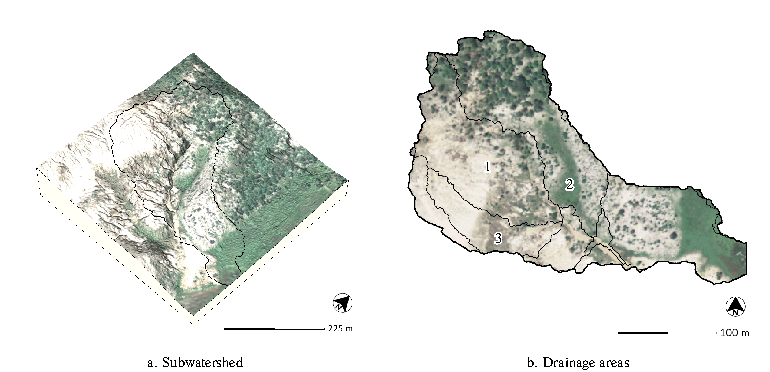
\includegraphics[width=\textwidth,height=0.95\textheight,keepaspectratio]{figures/watershed.pdf}
\caption{Subwatershed with 2014 orthoimagery
(a) draped over the 2016 digital elevation model
and (b) drainage areas with 2014 orthoimagery, Patterson Branch, Fort Bragg, NC, USA}
\label{fig:watershed}
\end{figure}

With 650~\unit{km}$^{2}$ of land
Fort Bragg is the largest military installation in the US
and has extensive areas of bare, erodible soils
on impact areas, firing ranges, landing zones, and dropzones. 
It is located in the Sandhills region of North Carolina 
with a Longleaf Pine and Wiregrass Ecosystem \citep{Sorrie2006}.
%
The study landscape 
-- a subwatershed of Patterson Branch (Figure~\ref{fig:watershed}) 
in the Coleman Impact Area --
is pitted with impact craters from artillery and mortar shells
and has an active, approximately 2~\unit{m} deep gully. 
%
It is a Pine-Scrub Oak Sandhill community
composed primarily of Longleaf Pine (\emph{Pinus palustris})
and Wiregrass (\emph{Aristida stricta})
on Blaney and Gilead loamy sands 
\citep{Sorrie2004}. 
%
Throughout the Coleman Impact Area
frequent fires ignited by live munitions
drive the ecological disturbance regime
of this fire adapted ecosystem.
%
In 2016 the  450~\unit{m}$^{2}$ study site was
43.24\% bare ground with predominately loamy sands,
39.54\% covered by the Wiregrass community, and
17.22\% forested with the Longleaf Pine community 
(Figure~\ref{fig:study_area}a). 
%
We hypothesize that the elimination of forest cover
in the impact zone
triggered extensive channelized overland flow,
gully formation, and sediment transport into the creek. 

% --------- DATA ---------
Timeseries of digital elevations models 
and landcover maps for the study landscape
were generated from lidar pointclouds and orthophotography.
%(Figure~\ref{fig:study_area}a-c). 
The digital elevations models for 2004, 2012, and 2016
were interpolated at 1~\unit{m} resolution
using the regularized spline with tension function \citep{Mitasova1993,Mitasova2005}
from airborne lidar surveys 
collected by the NC Floodplain Mapping program and Fort Bragg. 
%
Unsupervised image classification 
was used to identify clusters of spectral reflectance
in a timeseries of 1~\unit{m} resolution orthoimagery 
collected by the National Agriculture Imagery Program.
The landcover maps were derived from the
classified lidar point clouds and the classified orthoimagery.
Spatially variable soil erosion factors 
-- the k-factor, c-factor, Manning's coefficient, and runoff rate --
were then derived from the landcover and soil maps.
The dataset for this study is hosted at 
\url{https://github.com/baharmon/landscape\_evolution_dataset}
under the ODC Open Database License (ODbL).
The data is derived from publicly available data from
the US Army, USGS, USDA, Wake County GIS, NC Floodplain
Mapping Program, and the NC State Climate Office.
There are detailed instructions for preparing the input data in the 
\href{https://github.com/baharmon/landscape_evolution/blob/master/tutorial.md}{tutorial}
and a complete record of the commands used to process the sample data in the
\href{https://github.com/baharmon/landscape_evolution_dataset/blob/master/nc_spm_evolution/DATA.md}{data log}.

% --------- MORPHOLGY ---------
We used the geomorphons method 
of automated landform classification
based on the openness of terrain \citep{Jasiewicz2013}
and the difference between the digital elevation models 
to analyze the changing morphology of the study area
(Figures~\ref{fig:study_area} \& \ref{fig:study_area_detail}). 
%
The 2~\unit{m} deep gully -- 
its channels classified as valleys and 
its scour pits as depressions by geomorphons -- 
has multiple mature branches
and ends with a depositional fan.
%
The gully has also developed 
depositional ridges beside the channels.
Deep scour pits have developed 
where branches join the main channel 
and where the main channel has sharp bends.
%
A new branch has begun to form 
in a knickzone classified as a mix of valleys and hollows
on a grassy swale on the northeast side of the gully.
Between 2012 and 2016 a depositional ridge
developed at the foot of this nascent branch
where it would meet the main channel. 
%
The 2016 minus 2012 DEM of Difference (DoD) -- 
i.e.~ the difference in elevation 
(Figures~\ref{fig:study_area}c \& \ref{fig:study_area_detail}c) --
shows a deepening of the main channel 
by approximately 0.2~\unit{m} 
and scours pits by approximately 1~\unit{m},
while depositional ridges have formed and grown up to
approximately 1~\unit{m} high.
%
The DoD also shows that
244.60 \unit{m}$^3$ of sediment were deposited
on the depositional fan between 2012 and 2016.

% study area figure
\begin{figure}
\center
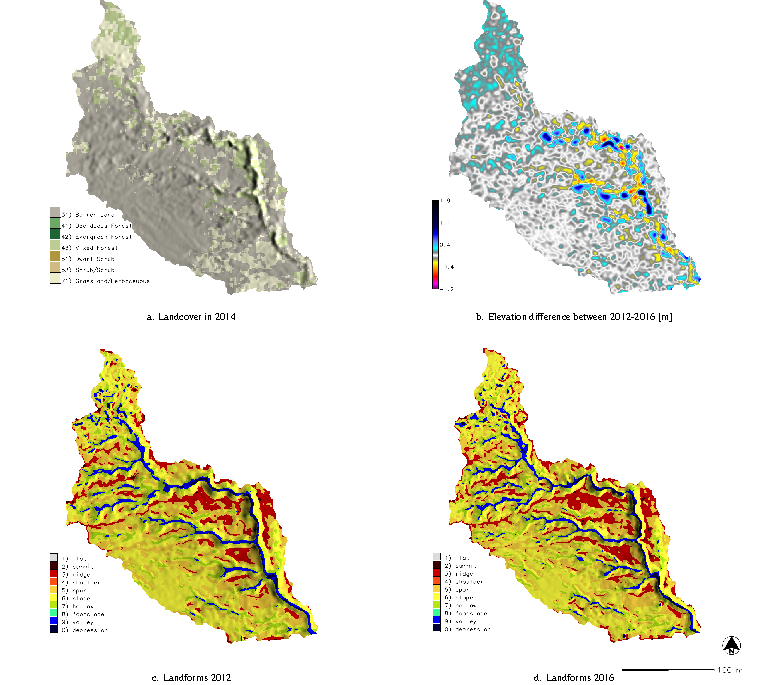
\includegraphics[width=\textwidth,height=0.95\textheight,keepaspectratio]{figures/study_area.pdf}
\caption{Morphological Change, Study Subwatershed, Patterson Branch, Fort Bragg, NC, USA.
(a) Landcover in 2014, 
(b) landforms in 2012,
(c) elevation difference between 2012-2016 [m], and
(d) landforms in 2016.
}
\label{fig:study_area}
\end{figure}

% study area figure detail
\begin{figure}
\center
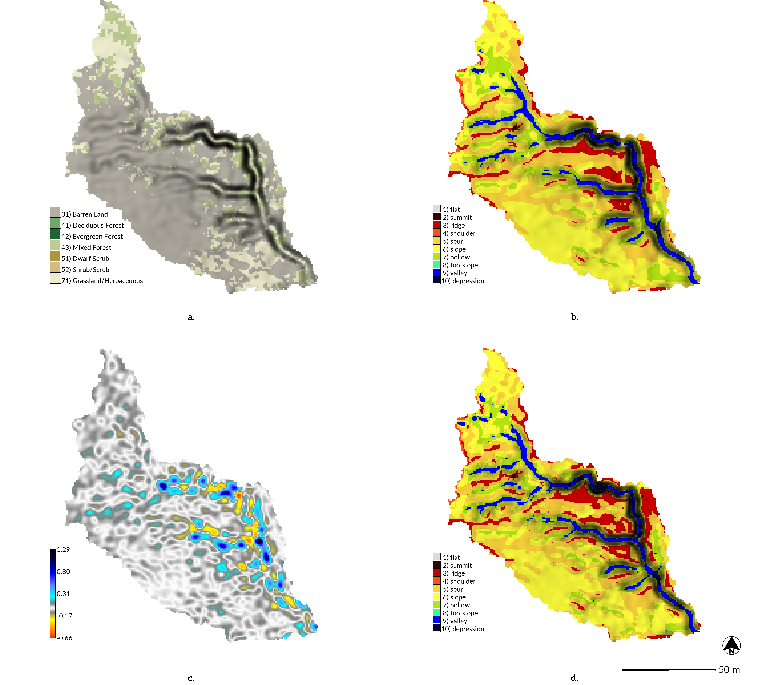
\includegraphics[width=\textwidth,height=0.95\textheight,keepaspectratio]{figures/study_area_detail.pdf}
\caption{Detailed Morphological Change, Drainage Area 1, Study Subwatershed, Patterson Branch, Fort Bragg, NC, USA.
(a) Landcover in 2014, 
(b) landforms in 2012,
(c) elevation difference between 2012-2016 [m], and
(d) landforms in 2016.
}
\label{fig:study_area_detail}
\end{figure}

% --------- SIMULATIONS ---------
\subsection{Simulations}
%
We ran a sequence of r.sim.terrain simulations 
with design storms
for the Patterson Branch subwatershed study area
to demonstrate the capabilities 
of the RUSLE3D, USPED, and SIMWE models
(Table~\ref{table:simulations}).
%
To analyze the results of the simulations,
we compared 
net differences in elevation
morphological features,
and volumetric change.
%
% design storms
While r.sim.terrain can use rainfall records,
we used design storms to demonstrate and test 
the basic capabilities of the model. 
Our design storms were based off the peak rainfall values
in records from the State Climate Office of North Carolina.
% parameters
We used RUSLE3D to simulate landscape evolution
in a dynamic, detachment capacity limited soil erosion regime
for a 120~\unit{min} design storm
with 3~\unit{min} intervals 
and a constant rainfall intensity of 50~\unit{mm~hr}$^{-1}$
(Figure~\ref{fig:rusle_simulation}).
%
We used USPED to simulate landscape evolution
in a dynamic, transport capacity limited soil erosion regime
for a 120~\unit{min} design storm
with 3~\unit{min} intervals 
and a constant rainfall intensity of 50~\unit{mm~hr}$^{-1}$
(Figure~\ref{fig:usped_simulation}).
%
We used SIMWE to simulate landscape evolution
in a steady state, variable erosion-deposition soil erosion regime
for a 120~\unit{min} design storm
with a constant rainfall intensity of 50~\unit{mm~hr}$^{-1}$
(Figure~\ref{fig:simwe_simulation}). 
%
In all of the simulations 
a sink filling algorithm
-- an optional parameter in r.sim.terrain -- 
was used to reduce the effects of positive feedback loops
that cause the over-development of scour pits. 

% scripts
The simulations were automated and run in parallel
using Python scripts that are available in the 
\href{https://github.com/baharmon/landscape_evolution}{software repository}.
% reproducibility
The simulations can be reproduced using these scripts
and the study area dataset 
by following the instructions 
in the Open Science Framework repository 
at \url{https://osf.io/tf6yb/}.
% benchmarks
The simulations were run 
in GRASS GIS 7.4 
on a desktop computer 
with 64-bit Ubuntu 16.04.4 LTS,
8 x 4.20 GHz Intel Core i7 7700K CPUs,
and 32 GB RAM. 
% multithreading
Simulations using SIMWE 
are far more computationally intensive
than RULSE3D or USPED, 
but support multi-threading 
when compiled with OpenMP. 
% runtime
Dynamic simulations of RUSLE3D and USPED took
2~\unit{min}~36~\unit{s} and 
3~\unit{min}~14~\unit{s} respectively
to run on a single thread, 
while the steady state simulation for SIMWE took 
44~\unit{min}~51~\unit{s} running on 6 threads
(Table~\ref{table:simulations}).

\subsection{Results}

% --------- RESULT TABLES ---------

% table of simulations
\begin{table*}
\small
\caption{Landscape evolution simulations}
\begin{tabu} to \textwidth {XXXXXllllX}
\toprule
Flow regime & Model & Intensity & Duration & Interval & m & n & $\rho_s$ & Threads & Runtime\\
\midrule
Dynamic & RUSLE3D & 50~\unit{mm~hr}$^{-1}$ & 120~\unit{min} & 3~\unit{min} &  0.4 & 1.3 & & & 2~\unit{min}~36~\unit{s}\\
Dynamic & USPED & 50~\unit{mm~hr}$^{-1}$ & 120~\unit{min} & 3~\unit{min} &  1.5 & 1.2 & 1.6 & & 3~\unit{min}~14~\unit{s}\\
Steady state & SIMWE & 50~\unit{mm~hr}$^{-1}$ & 120~\unit{min} & 120~\unit{min} & & & 1.6 & 6 & 44~\unit{min}~51~\unit{s}\\
\bottomrule
\\
\end{tabu}
\label{table:simulations} 
\end{table*}

% volumetric change table
\begin{table*}
\small
\caption{Volumetric change}
\begin{tabu} to \textwidth {lXXXl}
\toprule
Difference of DEMs (DoD) & Threshold [m] &  Erosion [m$^3$] & Deposition [m$^3$] & Net change [m$^3$]\\
\midrule
2016 - 2012 & $\pm$0.18 & 152.96 & 807.74 & 654.77\\
Simulated with RUSLE3D - 2012 & None & 1480.75 & 0 & -1480.75\\
Simulated with USPED - 2012 & None & 1235.08 & 727.46 & -507.62\\
Simulated with SIMWE -2012 & None & 758.56 & 608.91 & -149.66\\
\bottomrule
\\
\end{tabu}
\label{table:volumetric_change} 
\end{table*}

% --------------------------------------------

% volumetric change
We used the Difference in DEMs
to compute volumetric changes
between the lidar surveys
and the simulations
(Table~\ref{table:volumetric_change}).
We applied a threshold of $\pm$0.18 \unit{m}
to the lidar surveys since they had a
vertical accuracy at a 95\% confidence level
of 18.15~\unit{cm} 
based on a 9.25~\unit{cm} root mean square error (RMSEz) 
for non vegetated areas in accordance with 
the National Digital Elevation Program guidelines
\citep{NCLidar2018}.
%regime
Given the presence of the mature gully 
with ridges along its banks, 
we hypothesize that
the study landscape had previously been dominated by 
a detachment limited soil erosion regime, 
but -- given the net change of 654.77~\unit{m}$^3$ --
had switched to a transport capacity limited or 
variable erosion-deposition regime
during our study period. 

% rusle
The dynamic RUSLE3D simulation 
carved a deep incision 
in the main gully channel
where water accumulated
(Figure~\ref{fig:rusle_simulation}).
As a detachment capacity limited model
RUSLE3D's results were
dominated by erosion and 
thus negative elevation change.
It eroded 1480.75~\unit{m}$^3$ of sediment
with no deposition.

% usped
The dynamic USPED simulation
eroded the banks of the gully
and deposited in channels
causing the gully grow wider and shallower
(Figure~\ref{fig:usped_simulation}). 
% usped
As a transport capacity limited model
USPED generated a distributed pattern
with both erosion and deposition.
Erosion far exceeded deposition with
1235.08~\unit{m}$^3$ of sediment eroded 
and 727.46~\unit{m}$^3$ deposited
for a net change of -507.62~\unit{m}$^3$.
While USPED's pattern of elevation change
was grainy and fragmented, 
it captured the process of channel 
filling and widening expected with 
a transport capacity limited soil erosion regime.

% simwe
The steady state SIMWE simulation
for a variable erosion-deposition regime
predicted the morphological processes and features
expected of its regime including
gradual aggradation,
channel widening,
the formation of depositional ridges
along the thalweg of the channel,
and the development of the depositional fan
(Figure~\ref{fig:simwe_simulation}).
% volumetric change
SIMWE was the closest to the observed baseline
volumetric change.
It balanced erosion and deposition with 
785.56~\unit{m}$^3$ of sediment eroded
and 608.91~\unit{m}$^3$ deposited
for a net change of -149.66~\unit{m}$^3$.
% depositional fan
Only the SIMWE simulation deposited sediment
on the depositional fan. 
While the difference of lidar surveys showed
that 244.60~\unit{m}$^3$ of sediment 
were deposited on the fan,
SIMWE predicted that 54.05~\unit{m}$^3$
would be deposited.

% comparison of dynamic and steady state results
SIMWE was unique in simulating unsteady flows 
(Figure~\ref{fig:simwe_simulation}a)
and fine-scale geomorphological processes 
such as the development of depositional ridges 
and a depositional fan. 
%
While USPED generated a grainy pattern of erosion and deposition,
it was much faster than SIMWE 
(Table~\ref{table:simulations})
and still simulated 
the key morphological patterns and processes -- 
channel incision, filling, and widening. 
%
Given their speed
and approximate modeling of erosive processes, 
RUSLE3D and USPED 
are effective for simulating landscape evolution
on large rasters.
RUSLE3D for example has been used to
model erosion for the entire 650~\unit{km}$^{2}$ 
Fort Bragg installation at 9~\unit{m} resolution
\citep{Levine2018}. 

% rusle figure
\begin{figure}
\center
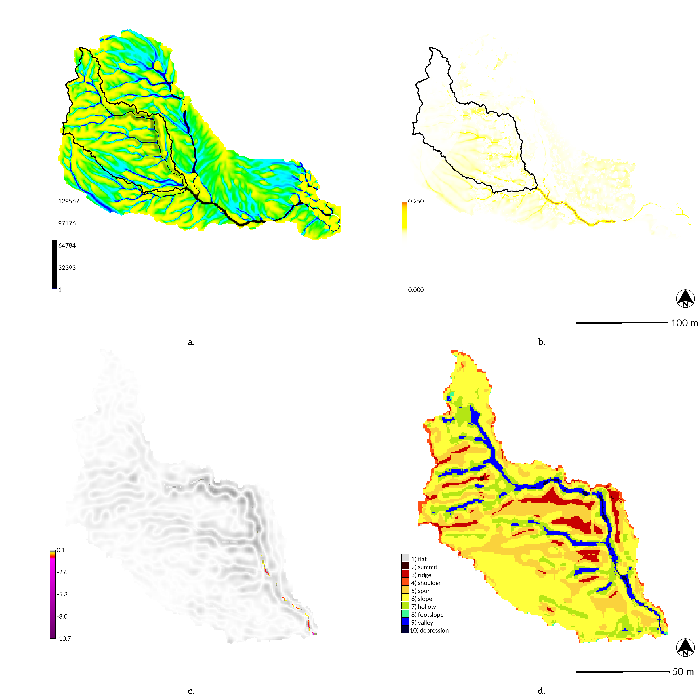
\includegraphics[width=\textwidth,height=0.925\textheight,keepaspectratio]{figures/rusle.pdf}
\caption{Dynamic simulation with RUSLE3D 
for a 120~\unit{min} event 
with a rainfall intensity of 50~\unit{mm~hr}$^{-1}$
at 1~\unit{m} resolution for
the Study Subwatershed (a-b)
and Drainage Area 1 (c-d)
on Patterson Branch, Fort Bragg, NC.
The (a) flow accumulation  and
(b) erosion [\unit{kg~m}$^{-2}$~\unit{s}$^{-1}$]
for the Study Subwatershed in the final 3~\unit{min} timestep.
The (c) net difference [\unit{m}] and (d) landforms 
for Drainage Area 1.
}
\label{fig:rusle_simulation}
\end{figure}

% usped figure
\begin{figure}
\center
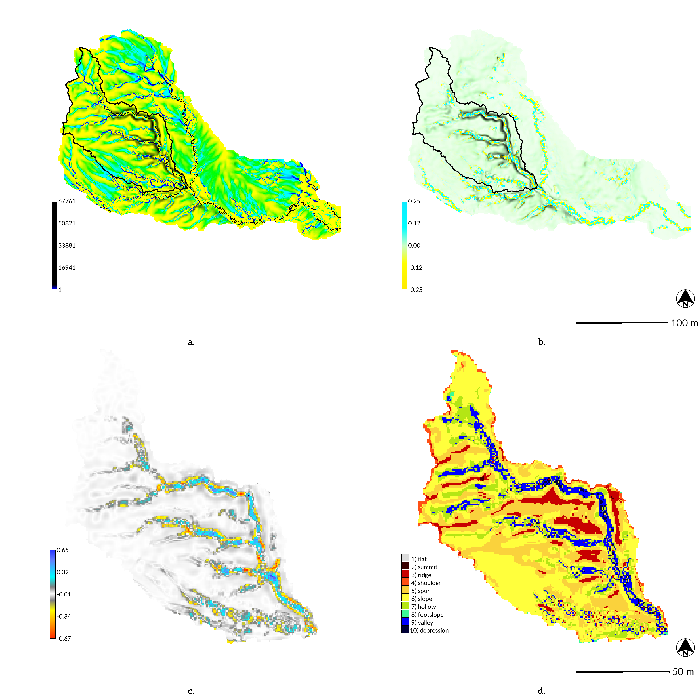
\includegraphics[width=\textwidth,height=0.925\textheight,keepaspectratio]{figures/usped.pdf}
\caption{Dynamic simulation with USPED
for a 120~\unit{min} event 
with a rainfall intensity of 50~\unit{mm~hr}$^{-1}$
at 1~\unit{m} resolution for
the Study Subwatershed (a-b)
and Drainage Area 1 (c-d)
on Patterson Branch, Fort Bragg, NC.
The (a) flow accumulation and
(b) erosion-deposition [\unit{kg~m}$^{-2}$~\unit{s}$^{-1}$]
for the Study Subwatershed in the final 3~\unit{min} timestep.
The (c) net difference [\unit{m}] and (d) landforms 
for Drainage Area 1.
}
\label{fig:usped_simulation}
\end{figure}

% steady state simwe figure
\begin{figure}
\center
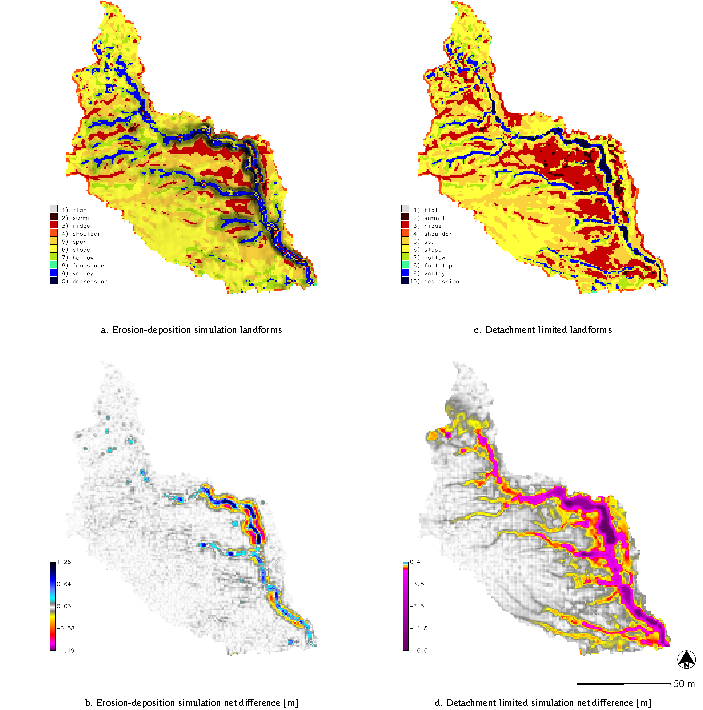
\includegraphics[width=\textwidth,height=0.95\textheight,keepaspectratio]{figures/simwe.pdf}
\caption{
Steady state SIMWE simulations 
for a 120~\unit{min} event 
with a rainfall intensity of 50~\unit{mm~hr}$^{-1}$
at 1~\unit{m} resolution for the
Study Subwatershed (a-b)
and Drainage Area 1 (c-d)
on Patterson Branch, Fort Bragg, NC.
The (a) depth of unsteady flow [\unit{m}] and
(b) erosion-deposition [\unit{kg~m}$^{-2}$~\unit{s}$^{-1}$]
for the Study Subwatershed.
The (c) net difference [\unit{m}] and (d) landforms
for Drainage Area 1.
}
\label{fig:simwe_simulation}
\end{figure}

% -------------------- Discussion ---------------------------------
\section{Discussion}

% limitations
Limitations of this landscape evolution model include
shallow overland flow, units, computation time, and raster size.
r.sim.terrain only models shallow overland flows, 
not fluvial processes or subsurface flows.
It requires data -- including 
elevation and rainfall intensity -- in metric units. 
The implementation of SIMWE in GRASS GIS
is computationally intensive 
and may require long computation times even with multithreading.
Because SIMWE uses a Green's function Monte Carlo solution 
of the sediment transport equation, 
the accuracy, detail, and smoothness of the results 
depend on the number of random walkers.
While a large number of random walkers will reduce the
numerical error in the path sampling solution,
it will also greatly increase computation time.
A customized compilation of GRASS GIS 
is needed to run SIMWE with more than 7 million random walkers.
This limits the size of rasters 
that can be easily processed with SIMWE,
while RUSLE3D and USPED are much faster, computationally efficient,
and can easily be run on much larger rasters. 

%It is challenging to quantitatively assess the performance of
%landscape evolution models at a watershed scale.
%While geomorphological statistics 
%like slope-area relationships and catchment hypsometry
%are used to assess model results \citep{Tucker2010}, 
%the drainage networks generated 
%may have similar statistics, 
%but very different spatial patterns \citep{Ijjasz1992}.
%Furthermore drainage networks 
%are sensitive to initial conditions
%with errors propagating exponentially over time
%\citep{Ijjasz1992}. 
%Measured versus simulated erosion and deposition values
%can be compared through landscape element classes 
%based on slope and contributing area
%\citep{Peeters2006,Temme2011}.

% future work
In the future we plan to assess this model
by comparing simulations against 
a monthly timeseries
of submeter resolution surveys
by unmanned aerial systems and terrestrial lidar. 
We also plan to develop a case study demonstrating
how the model can be used as a planning tool 
for landscape restoration. 
Planned enhancements to the model include 
modeling subsurface flows, 
accounting for bedrock, 
and a reverse landscape evolution mode
for backward modeling. 

% -------------------- CONCLUSIONS ---------------------------------
\conclusions

The short-term landscape evolution model 
r.sim.terrain can simulate the development of 
gullies, rills, and hillslopes by overland water erosion
for a range of hydrologic and soil erosion regimes.
The model is novel for simulating landscape evolution
based on unsteady flows. 
The landscape evolution model was tested
with a series of simulations for different 
hydrologic and soil erosion regimes
for a highly eroded sub-watershed on Fort Bragg
with an active gully.
For each regime it generated the 
morphological processes and features expected.
% physics based models
The physics-based SIMWE model 
simulated morphological processes 
for a variable erosion-deposition regime such as 
gradual aggradation, channel widening, 
scouring, the development of
depositional ridges along the thalweg,
and the growth of the depositional fan.
% empirical models
The empirical RUSLE3D model simulated channel incision
in a detachment limited soil erosion regime,
while the semi-empirical USPED model
simulated channel widening and filling
in a transport limited regime. 
% applications
Since r.sim.terrain is a GIS-based model that simulates 
fine-scale morphological processes and features,
it can easily and effectively be used 
in conjunction with other GIS-based tools
for geomorphological research,
land management and conservation,
erosion control, and landscape restoration. 

% --------------------CODE AND DATA------------------------

\codedataavailability{
% open science
As a work of open science
this study is reproducible, repeatable, and recomputable.
Since the data, model, GIS, dependencies are all 
free and open source, the study can easily be reproduced.
% code
The landscape evolution model 
has been implemented in Python as module
for GRASS GIS, a free and open source GIS.
 The source code for the model is hosted on GitHub at 
\url{https://github.com/baharmon/landscape_evolution}
under the GNU General Public License version 2.
The code repository also includes Python scripts 
for running and reproducing the simulations in this paper. 
The digital object identifier (DOI) 
for the version of the software documented in this paper is:
\url{https://doi.org/10.5281/zenodo.2542921}.
There are detailed instructions for running this model in the manual at
\url{https://grass.osgeo.org/grass76/manuals/addons/r.sim.terrain.html}
and the tutorial at
\url{https://github.com/baharmon/landscape_evolution/blob/master/tutorial.md}.
% data
The geospatial dataset for the study area is available on GitHub at
\url{https://github.com/baharmon/landscape_evolution_dataset}
under the 
\href{https://opendatacommons.org/licenses/odbl/}{Open Database License} 
with the DOI:
\url{https://doi.org/10.5281/zenodo.2542929}.
The
\href{https://github.com/baharmon/landscape_evolution_dataset/blob/master/nc_spm_evolution/DATA.md}{data log} has a complete record of the commands used to process the sample data.
% osf
The source code, scripts, data, and results are also hosted
on the Open Science Framework at 
\url{https://osf.io/tf6yb/}
with the DOI:
\url{https://doi.org/10.17605/osf.io/tf6yb}.
}

% ----------------------------------------------------------------------------

\noappendix 

\authorcontribution{
Brendan Harmon developed 
the models, code, data, case studies, and manuscript.
Helena Mitasova contributed to the development 
of the models and case studies and revised the manuscript.
Anna Petrasova and Vaclav Petras
contributed to the development of the code.
All authors read and approved the final manuscript.
}

\competinginterests{The authors declare that they have no conflict of interest.} 

\begin{acknowledgements}
We acknowledge the GRASS GIS Development Community
for developing and maintaining GRASS GIS.
\end{acknowledgements}

% ---------------------REFERENCES---------------------------
\bibliographystyle{copernicus}
\bibliography{landscape_evolution.bib}

\end{document}
